\begin{titlepage}
%
%~\\[1cm]
%régler l'épaisseur des lignes
\newcommand{\HRule}{\rule{\linewidth}{0.5mm}}

\begin{center}
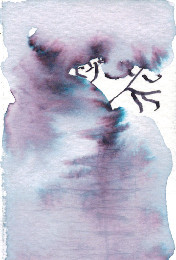
\includegraphics[scale=0.5]{./presentation/gauche}
\hspace{1cm}
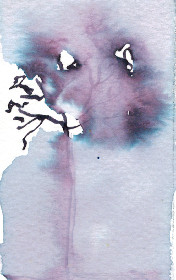
\includegraphics[scale=0.5]{./presentation/droite}
\end{center}

\textsc{\Large }\\[0.5cm]

% Title \\[0.4cm]
\HRule

\begin{center}
{\Huge \bfseries  Croyance, doute\\
et opinion\\[0.4cm] }
\end{center}

\HRule \\[1.5cm]


\vfill

\begin{flushright} \huge
%\emph{Auteur:}\\
%Stephan \textsc{Runigo}
Extraits de dictionnaires
\end{flushright}

\vfill
{\sf
\begin{itemize}[leftmargin=1cm, label=\ding{32}, itemsep=1pt]
\item {\bf Objet : } {\it Croyance, doute et opinion} en philosophie.
\item {\bf Contenu : } Définitions et article encyclopédique.
\item {\bf Public concerné : } Philosophe en herbe.
\end{itemize}
}

\vfill

% Bottom of the page
{\large \today}

\end{titlepage}
